\documentclass[../main]{subfiles}
\begin{document}

\chapter{模拟乘法器调幅及同步检波实验}%
\label{cha:模拟乘法器调幅及同步检波实验}

\section{实验目的}%
\label{sec:\arabic{chapter}实验目的}

\begin{enumerate}

	\item 掌握用集成模拟乘法器实现全载波调幅、抑止载波双边带调幅和单边带调幅
		的方法。

	\item 研究已调波与调制信号以及载波信号的关系。

	\item 掌握调幅系数的测量与计算方法。

	\item 通过实验对比全载波调幅、抑止载波双边带调幅和单边带调幅的波形。

\end{enumerate}

\section{基本原理}%
\label{sec:\arabic{chapter}基本原理}

幅度调制就是载波的振幅(包络)随调制信号的参数变化而变化。本实验中载波是由高频信
号源产生的\SI{465}{\kHz}高频信号,\SI{10}{\kHz}的低频信号为调制信号。振幅调制器
即为产生调幅信号的装置。

用MC1496集成电路构成的调幅器电路图如图\ref{fig:调幅器电路图}所示。

\begin{figure}[htbp]
	\centering
	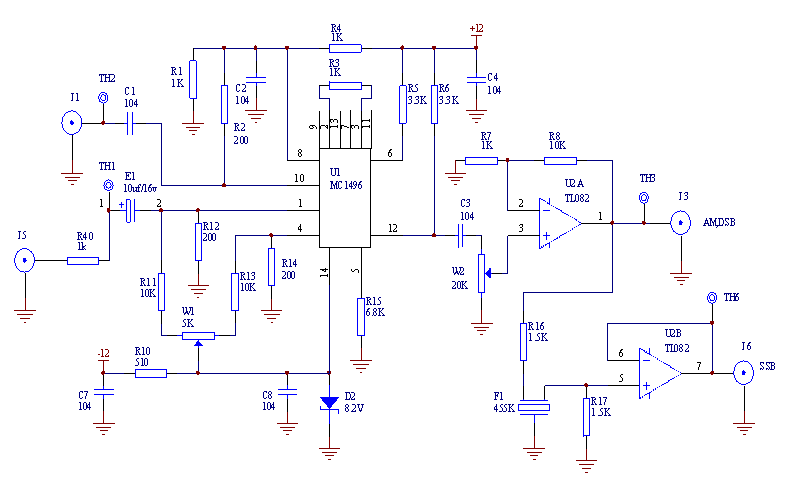
\includegraphics[width=0.8\linewidth]{mo.png}
	\caption{调幅器电路图}
	\label{fig:调幅器电路图}
\end{figure}

图中$ W_1 $用来调节引出脚1、4之间的平衡,器件采用双电源方式供电(\SI{+12}{\V})
,\SI{-8}{\V}),所以5 脚偏置电阻$ R_{15} $接地。电阻$ R_1 $、$ R_2 $、$ R_4 $、
$ R_5 $、$ R_6 $ 为器件提供静态偏置电压,保证器件内部的各个晶体管工作在放大状态
。载波信号加在$ V_1 - V_4 $的输入端,即引脚8 、 10之间;载波信号$ V_\mathrm{c} $
经高频耦合电容$ C_1 $从 10 脚输入,$ C_2 $ 为高频旁路电容,使 8 脚交流接地。调制
信号加在差动放大器$ V_5 $、$ V_6 $的输入端,即引脚1、4之间,调制信号$
V_\mathrm{\Omega} $经低频偶合电容$ E_1 $从1 脚输入。2、3 脚外接\SI{1}{\kohm}电阻
,以扩大调制信号动态范围。当电阻增大,线性范围增大,但乘法器的增益随之减小。已调
制信号取自双差动放大器的两集电极(即引出脚 6、 12之间)输出。

\section{实验步骤}%
\label{sec:\arabic{chapter}实验步骤}

\begin{enumerate}

	\item 全载波振幅调制$ m = \dfrac{V_\mathrm{mmax} - V_\mathrm{mmin}}
		{V_\mathrm{mmax} + V_\mathrm{mmin}} $ ,$ J_1 $ 端输入载波信号 $
		V_c(t) $ ,$ f_\mathrm{c} = \SI{465}{\kHz} $ , $ V_\mathrm{CP -
		P} = \SI{500}{\mV} $,再从$ J_5 $端口输入调制信号,其$
		f_\mathrm{\Omega} = \SI{10}{\kHz} $,当$ V_\mathrm{\Omega P-P} $
		由零逐渐增大时,则输出信号$ V_\mathrm{O}(t) $的幅度发生变化,最
		后出现如图 \ref{fig:普通调幅波波形}所示的有载波调幅信号的波形,
		记下AM波对应$ V_\mathrm{mmax} $ 和$ V_\mathrm{mmin} $,并计算调
		幅度$ m $。

		\begin{figure}[htbp]
			\centering
			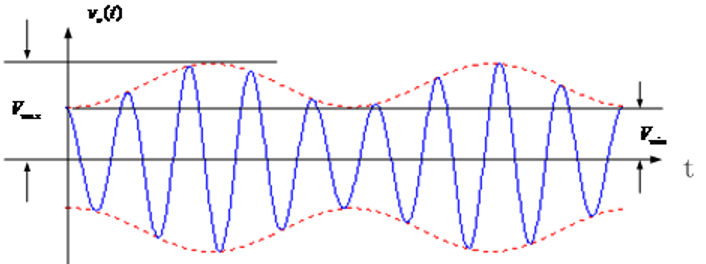
\includegraphics[width=0.8\linewidth]{wave.png}
			\caption{普通调幅波波形}
			\label{fig:普通调幅波波形}
		\end{figure}

	\item 集成电路(乘法器)构成解调器,解调全载波信号。

		在保持调幅波输出的基础上,将调幅波和高频载波输入解调乘法器$
		J_\mathrm{11} $和$ J_8 $端,用示波器观测解调器的输出,记录其频率和幅度。

		\begin{figure}[htbp]
			\centering
			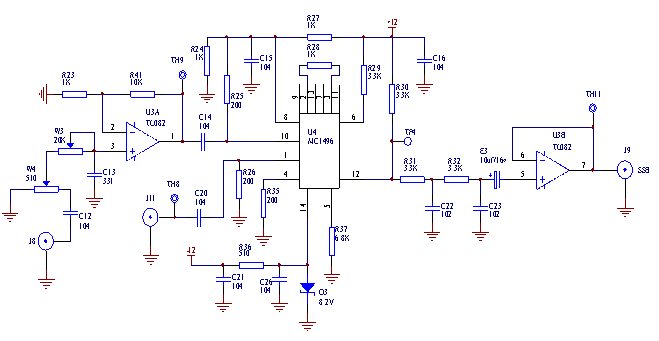
\includegraphics[width=0.8\linewidth]{dem.png}
			\caption{解调器电路图}
			\label{fig:解调器电路图}
		\end{figure}

\end{enumerate}

\section{实验报告要求}%
\label{sec:\arabic{chapter}实验报告要求}

\begin{Exercise}

	画出调幅实验中$ m = 30\% $、$ m = 50\% $、$ m = 80\% $的调幅波形,分析
	过调幅的原因。

\end{Exercise}

\begin{Answer}

	\begin{description}

		\item[调制度$ m = 0.3 $] 从图\ref{fig:0.3}可以看出,AM 调幅波的
			波峰值为 \SI{496}{\mV},波谷值为\SI{264}{\mV},所以调制
			度的计算值为 $ m = \dfrac{648 - 352}{648 + 352} = 0.3 $
			。

		\item[调制度$ m = 0.5 $] 从图\ref{fig:0.5}可以看出,AM 调幅波的
			波峰值为 \SI{584}{\mV},波谷值为 \SI{192}{\mV},所以调制
			度的计算值为$ m = \dfrac{768 - 240}{768 + 240} = 0.5 $。

		\item[调制度$ m = 0.8 $] 从图\ref{fig:0.8}可以看出,AM 调幅波的
			波峰值为 \SI{680}{\mV},波谷值为 72mV,所以调制度的计算
			值为 $ m = \dfrac{940 - 120}{940 + 120} = 0.8 $。

	\end{description}

\end{Answer}

\begin{figure}[htbp]
	\centering
	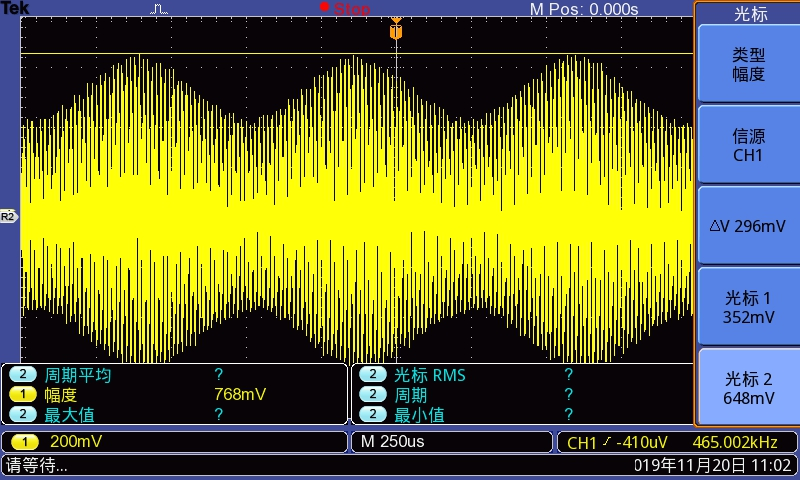
\includegraphics[width=0.8\linewidth]{3.jpg}
	\caption{$ m = 0.3 $}
	\label{fig:0.3}
\end{figure}

\begin{figure}[htbp]
	\centering
	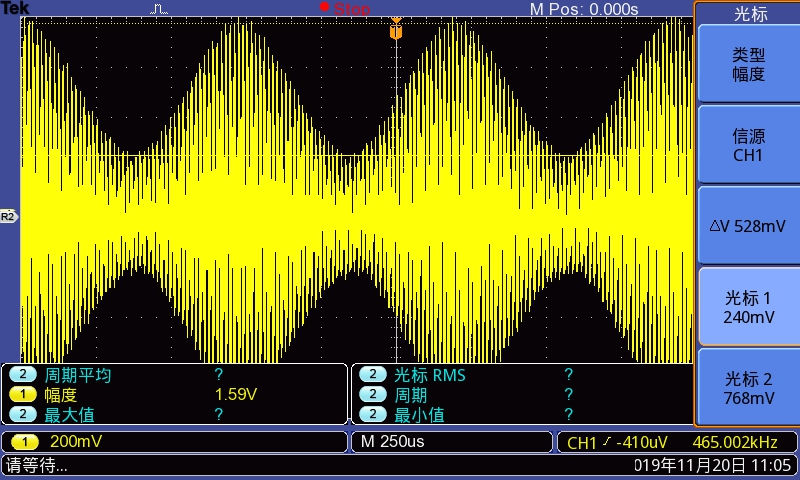
\includegraphics[width=0.8\linewidth]{5.jpg}
	\caption{$ m = 0.5 $}
	\label{fig:0.5}
\end{figure}

\begin{figure}[htbp]
	\centering
	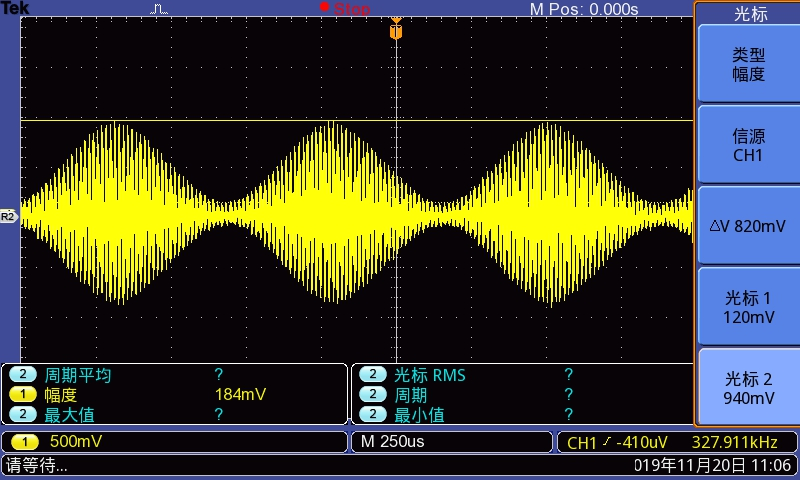
\includegraphics[width=0.8\linewidth]{8.jpg}
	\caption{$ m = 0.8 $}
	\label{fig:0.8}
\end{figure}

\begin{Exercise}

	画出全载波调幅波形、抑止载波双边带调幅波形及单边带调幅波形,比较三者区别
	。

\end{Exercise}

\begin{Answer}

	解调后的波形如图\ref{fig:解调后的波形}所示,解调后的频率如
	\ref{fig:解调后的频率}所示,接线图如图 \ref{fig:接线图}所示。

\end{Answer}

\begin{figure}[htbp]
	\centering
	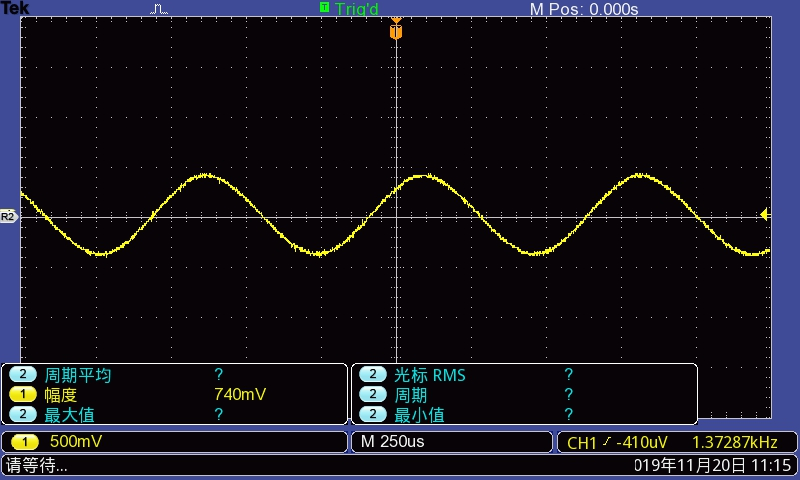
\includegraphics[width=0.8\linewidth]{wave.jpg}
	\caption{解调后的波形}
	\label{fig:解调后的波形}
\end{figure}

\begin{figure}[htbp]
	\centering
	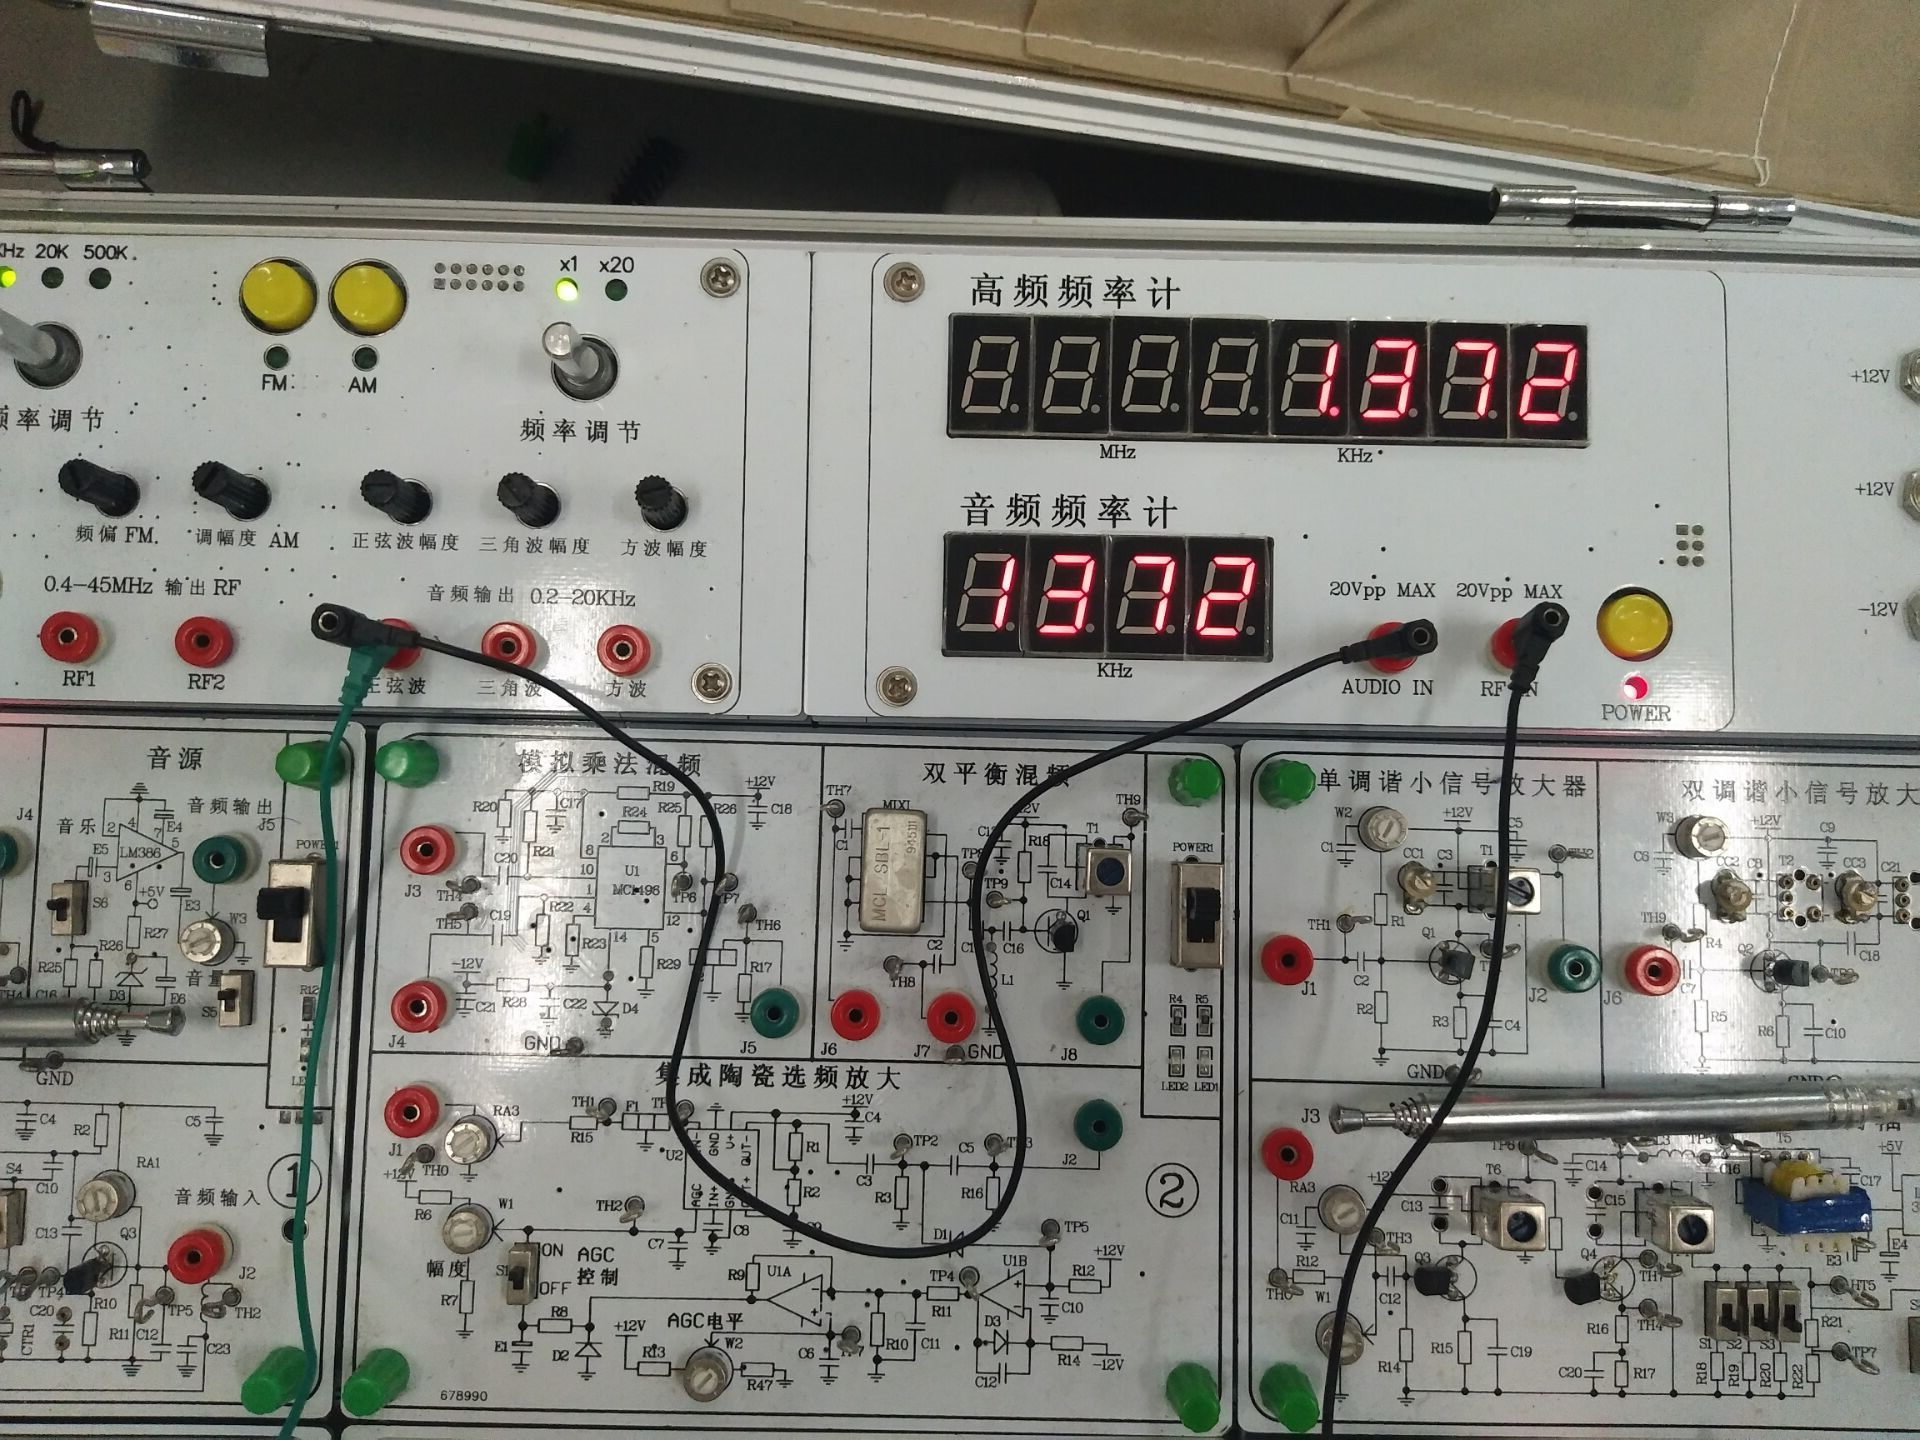
\includegraphics[width=0.8\linewidth]{freq.jpg}
	\caption{解调后的频率}
	\label{fig:解调后的频率}
\end{figure}

\begin{figure}[htbp]
	\centering
	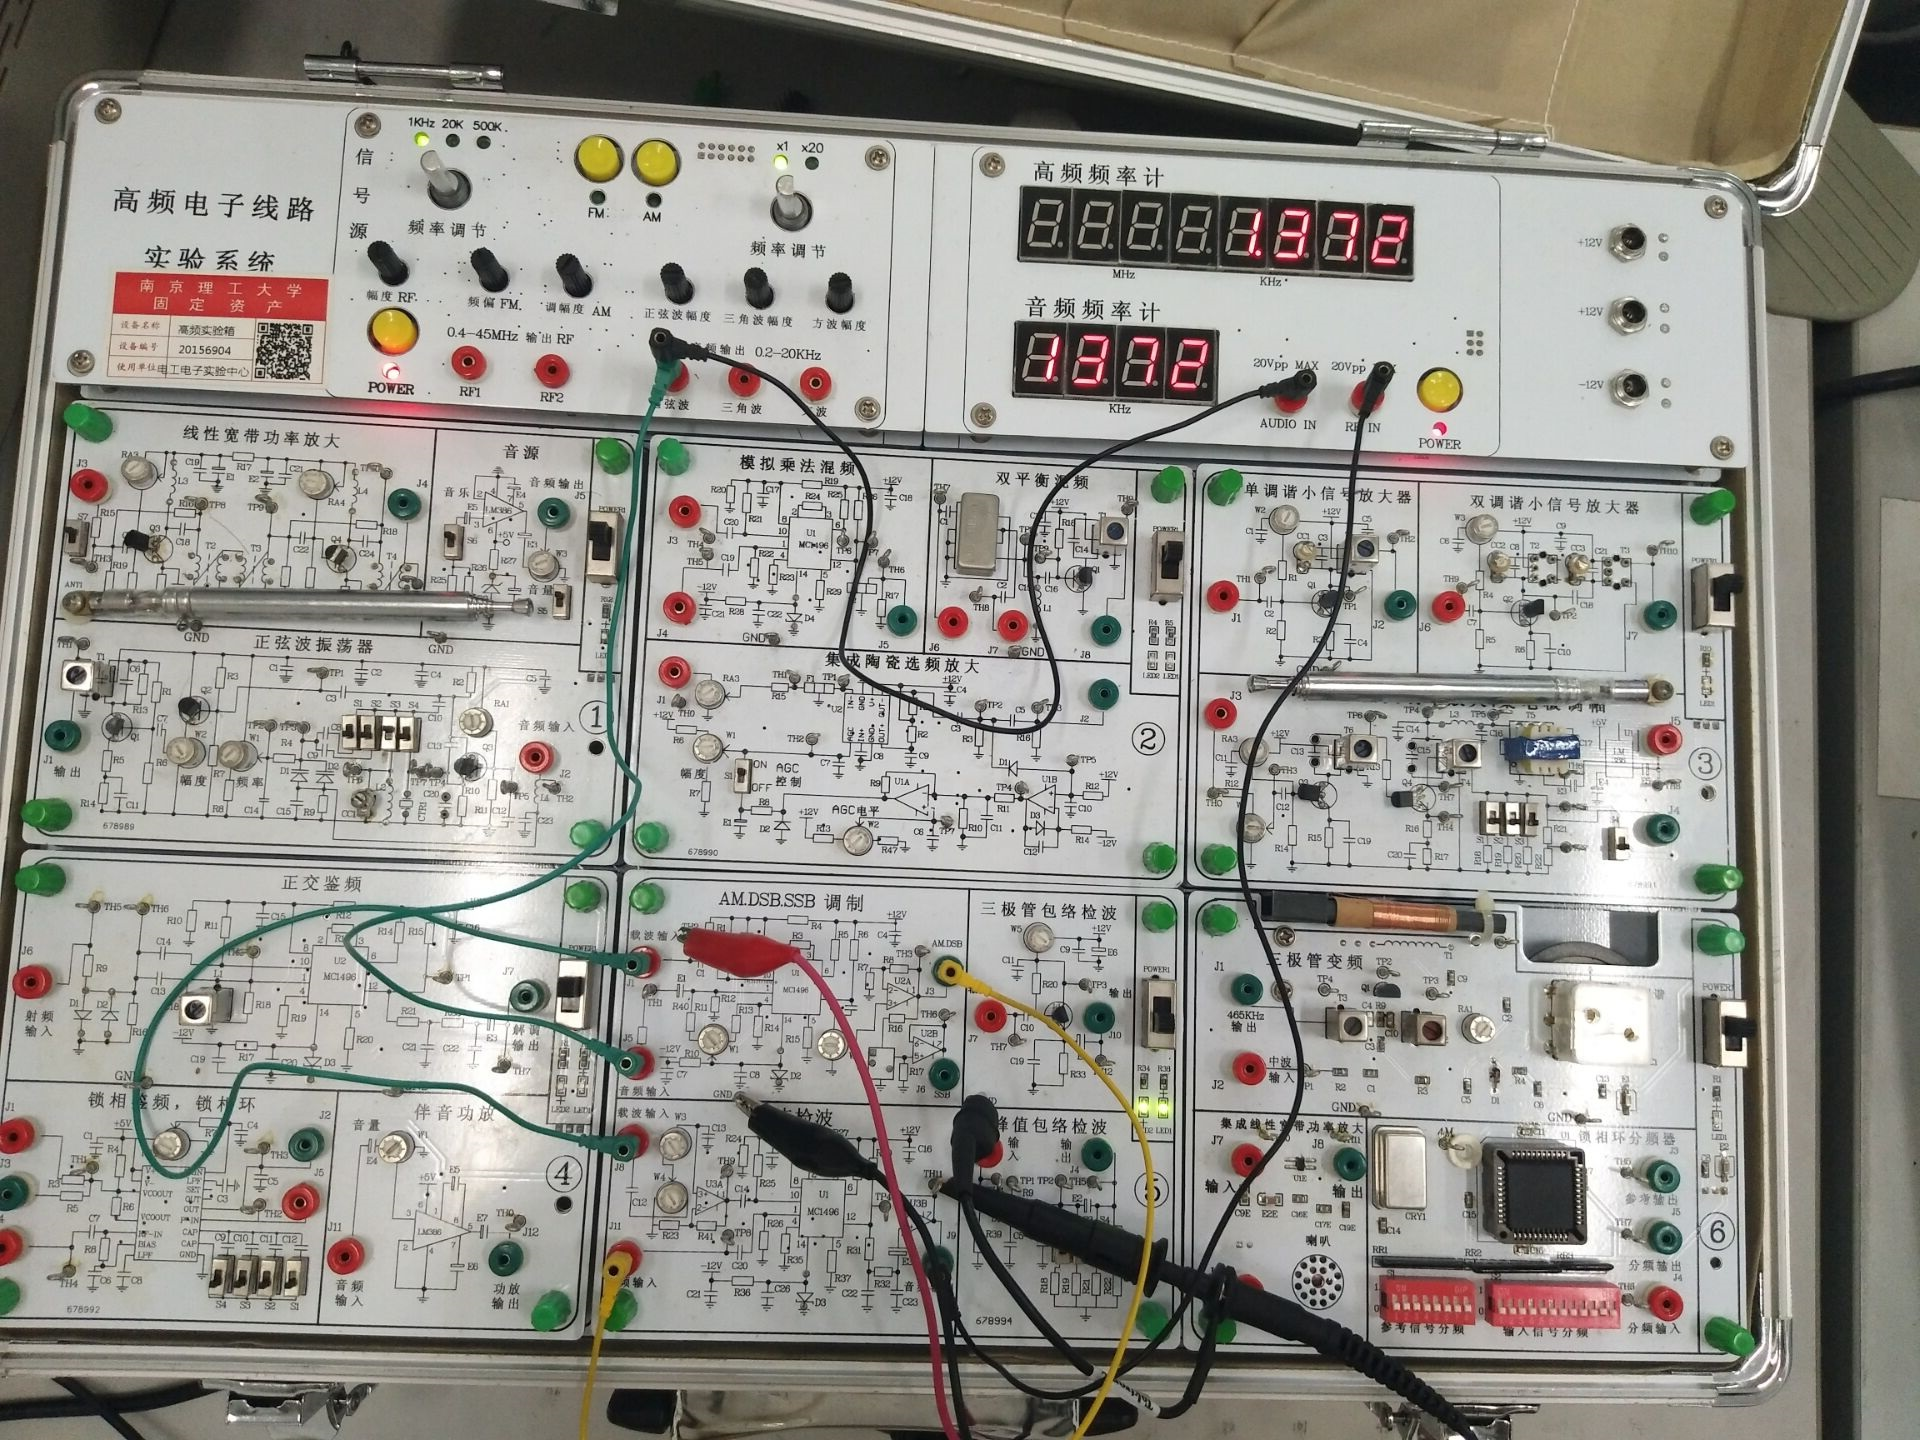
\includegraphics[width=0.8\linewidth]{circuit.jpg}
	\caption{接线图}
	\label{fig:接线图}
\end{figure}

\section{实验仪器}%
\label{sec:\arabic{chapter}实验仪器}

\begin{table}[htbp]
	\centering
	\caption{实验仪器}
	\label{tab:\arabic{chapter}实验仪器}
	\csvautobooktabular{tab/\arabic{chapter}/BOM.csv}
\end{table}

\end{document}

